% !TEX root = main.tex
\section{Narzędzie do monitorowania GenericMonitoringTool}
Wynikiem zmian w module AthenaMonitoring i kodzie algorytmów monitorowanych jest klasa GenericMonitoringTool.
Agreguje ona funkcjonalności zidentyfikowane jako kluczowe dla monitoringu, czyli możliwość deklaracji histogramów oraz wypełnianie ich wartościami zmiennych monitorowanych obliczonych w algorytmach.
Jednak w przeciwieństwie do pierwotnej implementacji, dostarcza ona kilka poziomów abstrakcji, umożliwiających centralizację połączenia pomiędzy tymi dwiema warstwami.
Nowa implementacja wprowadziła wiele rozwiązań, które sprawiły, że kod stał się bardziej czytelny, elastyczny i łatwiejszy w użyciu.
Moduł AthenaMonitoring jest przykładem kodu, który łatwiej jest przepisać, z wykorzystaniem fragmentów starego kodu, niż refaktoryzować. 

Największym zyskiem z tych zmian jest oddzielenie kodu zarządzającego cyklem życia obiektów ROOT od kodu algorytmów. 
Pozwoliło to zredukować ich objętość i umożliwiło osobom implementującym algorytmy skupienie się na ich głównym zadaniu, zamiast na obsłudze histogramów.
Dodatkowo sprawia to, że kod monitoringu stał się scentralizowany, dzięki czemu możliwe stały się aktualizacje ROOT, bez potrzeby modyfikowania już istniejących algorytmów.

Z wykorzystaniem GenericMonitoringTool możliwe stało się rozwiązanie problemu scalania histogramów.
Jest to konsekwencją tego, że w nowym rozwiązaniu istnieje centralny punkt w którym obsługiwane są histogramy.
Zatem łatwe stało się dodanie zabezpieczeń dla wywołań wielowątkowych w postaci użycia `mutex`ów.
Zapewniają one spójność danych wpisywanych do obiektów ROOT, a mają przy tym bardzo mały narzut czasowy.

Wdrożone warstwy abstrakcji, umożliwiły łatwiejsze dodawanie nowych funkcjonalności, które mogą realizować bardzo złożone scenariusze wypełniania histogramów.
Dobrym przykładem jest tu klasa LumiblockHistogramProvider, która realizuje funkcjonalność podziału danych na postawie kontekstu w jakim zostały one wygenerowane. 
Zaimplementowanie jej funkcjonalności w starej konwencji byłoby bardzo trudnym zadaniem. 

Dodatkowym zyskiem z takiego rozdzielenia odpowiedzialności i wprowadzenia kilku warstw abstrakcji jest możliwość łatwego tworzenia testów jednostkowych. 
Znacznie podniosło to jakość kodu pisanego na potrzeby monitoringu, przyśpieszyło jego proces powstawania oraz pozwoliło na wcześniejsze wykrywanie problemów.
Spowodowane jest to tym, że dla nowego rozwiązania, nie ma konieczności uruchamiania kosztownych czasowo algorytmów, aby przetestować kod.

\subsection{Wydajność wielowątkowa}

\begin{figure}[!ht]
\centering
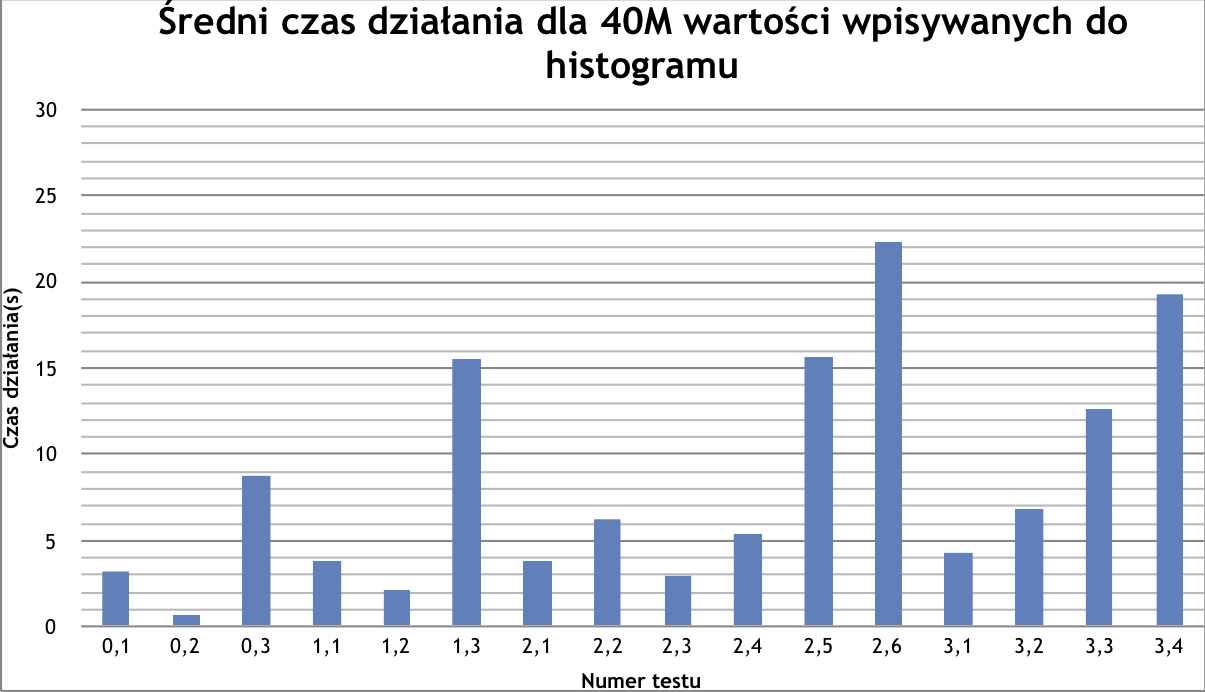
\includegraphics[width=1\textwidth]{img/avg_run_time.png}
\caption{
Wszystkie wyniki są średnią z 10 uruchomień.
0 - czas losowania 40M danych; 
1 - bezpośrednie wypełnianie histogramu z algorytmu;
2 - zmienna monitorowana bez synchronizacji wątków;
3 - zmienna monitorowana z synchronizacją wątków;
0,1 - jeden wątek;
0,2 - 800 wątków;
0,3 - 800 wątków + mutex;
1,1 - jeden wątek;
1,2 - 800 wątków, kompletność danych 5,15\%;
1,3 - 800 wątków + mutex;
2,1 - jeden wątek, histogram utworzony raz;
2,2 - jeden wątek, histogram tworzony za każdym razem;
2,3 - 800 wątków, histogram utworzony raz, kompletność danych 9,6\%;
2,4 - 800 wątków, histogram tworzony za każdym razem, kompletność danych 4,48\%;
2,5 - 800 wątków + mutex, histogram utworzony raz;
2,6 - 800 wątków + mutex, histogram tworzony za każdym razem;
3,1 - jeden wątek, histogram utworzony raz;
3,2 - jeden wątek, histogram tworzony za każdym razem;
3,3 - 800 wątków, histogram utworzony raz;
3,4 - 800 wątków, histogram tworzony za każdym razem;
}
\label{fig:athena:avgRunTime}
\end{figure}

Podczas implementacji zabezpieczeń przetwarzania wielowątkowego dla GenericMonitoringTool, bardzo ważne było sprawdzenie jak duży jest narzut na synchronizacje wątków. 
Przetestowane zostało kilka rozwiązań, w czego rezultacie najlepsze okazało się zastosowanie `mutex`'a z biblioteki standardowej C++ wewnątrz zmiennej monitorowanej. 
\figref{fig:athena:avgRunTime} prezentuje wyniki tych testów. 
W ich przypadku, czas działania algorytmu jest pomijalnie mały, gdyż jest w nich losowana pojedyncza wartość liczbowa.
W rzeczywistym użyciu spodziewane jest, że czas wykonywania algorytmu będzie dużo większy od czasu potrzebnego na obsługę sekcji krytycznej. 
Najbardziej reprezentatywne na tym wykresie są przypadki 1,3 oraz 3,3.

1,3 jest wynikiem działania kodu, który wykorzystuje mechanizmy dostępne przed refaktoryzacją.
Użytkownik samemu obsługuje synchronizacje z wykorzystaniem mutex'a dla 800 wątków i wypełnia histogram odwołując się bezpośrednio do obiektów frameworka ROOT.

3,3 jest wynikiem działania kodu wykorzystującego zmienną monitorowaną, która w sposób niewidoczny dla użytkownika dba o synchronizację i wypełnienie histogramów ROOT. 

Testy były przeprowadzane na wirtualizowanym środowisku LXPLUS~\cite{cern-lxplus}, które jest współdzielone między wieloma użytkownikami, co może obciążać te wyniki błędem. 
Jednak najważniejszy wniosek z nich jest taki, że GenericMonitoringTool nie wprowadza znaczącego narzutu na obsługę histogramów w porównaniu do podejścia bezpośredniego.
Różnica w czasie wykonania na korzyść zmiennej monitorowanej może być również spowodowana optymalizacjami dokonanymi przez kompilator. 

\subsection{Testy jednostkowe}
Jednym z wymogów przy tworzeniu nowego kodu do monitoringu było to, że musi on posiadać testy jednostkowe.
Aby to osiągnąć, został on zaprojektowany w sposób umożliwiający jego testowanie - wprowadzenie interfejsów i klas bazowych, oraz użycie wstrzykiwania zależności.
Pozwala to odizolować kod który chcemy zweryfikować i napisać testy które opiszą oczekiwane od niego zachowanie.

Athena dostarcza podstawowe narzędzia do tworzenia testów jednostkowych, takie jak np. asercje, jednak nie definiuje ona ich struktury.
Aby to usystematyzować powstał szablon pliku z testami dla kodu monitoringu, przedstawiony został na \lstref{lst:athena:unit_test_template}.

\lstinputlisting[
	style=cpp, 
	caption=Szablon pliku z testami jednostkowymi, 
	label={lst:athena:unit_test_template}
]{ExampleClassTestSuite.cxx}

Szablon podzielony jest na następujące sekcje:
\begin{itemize}
\item Zarejestrowane testy - w tej części, użytkownik jest zobowiązany do zadeklarowania testów, które mają zostać uruchomione. Wykorzystane jest tutaj makro `REGISTER\_TEST\_CASE`, którego celem jest uproszczenie tego procesu. Jej istnienie wynika z ograniczeń języka C++, który nie pozwala pobrać listy wszystkich dostępnych metod dla danej klasy.
\item Kod testów - definiuje ona metody `beforeEach` - wywoływana przed każdym testem - i `afterEach` - wywoływana po każdym teście. W razie potrzeby, użytkownik powinien w nich odpowiednio przygotować środowisko do testów. W tej sekcji użytkownik definiuje metody, które posłużą do weryfikacji poprawności zachowania testowanej klasy. Ich nazwa powinna zaczynać się od `test\_should`.
\item Metody pomocnicze - miejsce na metody pomocnicze zdefiniowane przez użytkownika na potrzeby testów.
\item Inicjalizacja i uruchomienie - w tej sekcji zdefiniowany jest sposób uruchomienia testów.
\item Rejestracja testów - tej części metody testowe są przygotowywane do uruchomienia. Użytkownik nie powinien jej modyfikować.  
\item Pola klasy - zawiera deklaracje wszystkich zmiennych. `m\_testObj` jest specjalną zmienną, która zawiera obiekt testowanej klasy.  
\end{itemize}

Szablon ten został wykorzystany na potrzeby przetestowania wszystkich najważniejszych komponentów GenericMonitoringTool.

\begin{cpp}[caption=Jeden z testów zdefiniowanych w ramach HistogramFactoryTestSuite~\cite{histogram-factory-test-suite}, label={lst:athena:histogram_factory_test_suite}]
void test_shouldRegisterAndReturnTH1DHistogram() {
   TH1D* const histogram = createHistogram<TH1D>("TH1D");
   VALUE(m_histSvc->exists("/HistogramFactoryTestSuite/TH1D")) EXPECTED(true);
   VALUE(histogram) NOT_EXPECTED(nullptr);
}
\end{cpp}

W celu poprawnego odizolowania testowanego kodu, powstały klasy dostępne tylko na potrzeby testów - `mocki`, których zadaniem jest imitowanie prawdziwych komponentów GenericMonitoringTool.
Ich zachowanie jest całkowicie pod kontrolą użytkownika.
Takie obiekty, w połączeniu ze wstrzykiwaniem zależności, umożliwiają całkowite uniezależnienie weryfikowanego kodu od innych komponentów.
